Devido à alta diferença de escala nos dados da lista \verb|varNum|, é necessária a realização de um reescalonamento destas variáveis. Primeiro, podemos aplicar uma transformação logarítmica nas variáveis \verb|L| e \verb|R| devido à grande assimetria dos dados nelas contidos, onde somamos uma quantidade insignificante $1.0 \cdot 10^{-10}$ para evitar possíveis casos de $\log(0)$ (que não ocorrem aqui, mas é importante se considerar).
\begin{longlisting}
    \begin{minted}{py}
        dSNum = dS[varNum].copy()
        
        dSNum['L'] = np.log10(dSNum['L'] + 1e-10) 
        dSNum['R'] = np.log10(dSNum['R'] + 1e-10) 
    \end{minted}
\end{longlisting}

Em seguida, podemos de fato fazer o reescalonamento das variáveis, onde será usado o método \verb|StandardScaler()|, afim de padronizar a média em 0 e a variância em 1. A escolha deste método é devido à sua adequação para aplicação do PCA e da clusterização, lidando bem com distribuições não normais e possíveis \textit{outliers}.
\begin{longlisting}
    \begin{minted}{py}
        from sklearn.preprocessing import StandardScaler
        
        scaler = StandardScaler()
        scaledNum = scaler.fit_transform(dSNum)
        scaledNumdS = pd.DataFrame(scaledNum, columns = varNum)
        
        X = pd.concat([scaledNumdS, encodeddS], axis = 1)
    \end{minted}
\end{longlisting}
onde agora, \verb|X| é a tabela \verb|dS| com as variáveis numéricas reescalonadas e com as variáveis categóricas agora codificadas em valores binários, sendo então uma tabela com 240 linhas e 18 colunas
\begin{table}[H]
    \centering
    \begin{tabular}{ccccccc}
        \toprule
        \verb|index| & \verb|Temperature| & \verb|L| & \verb|R| & $\cdots$ & \verb|Spectral_Class_M| & \verb|Spectral_Class_O|  \\ 
        \midrule
        0 & -0.779382 & -0.888096 & -0.950995 & $\cdots$ & 1.0 & 0.0 \\
        1 & -0.782110 & -1.061480 & -0.974683 & $\cdots$ & 1.0 & 0.0 \\
        2 & -0.828477 & -1.117944 & 0.602446 & $\cdots$ & 1.0 & 0.0 \\
        3 & -0.807496 & -1.16276 & -0.965717 & $\cdots$ & 1.0 & 0.0 \\
        4 & -0.897819 & -1.203776 & 0.604815 & $\cdots$ & 1.0 & 0.0 \\
        $\cdots$ & $\cdots$ & $\cdots$ & $\cdots$ & $\cdots$ & $\cdots$ & $\cdots$ \\
        235 & 2.983743 & 1.197284 & 1.230755 & $\cdots$ & 0.0 & 1.0 \\
        236 & 2.133913 & 1.285690 & 1.199858 & $\cdots$ & 0.0 & 1.0 \\
        237 & -0.175029 & 1.237125 & 1.242467 & $\cdots$ & 0.0 & 0.0 \\
        238 & -0.132438 & 1.205825 & 1.182580 & $\cdots$ & 0.0 & 0.0 \\
        239 & 2.872754 & 1.170775 & 1.297235 & $\cdots$ & 0.0 & 1.0 \\
        \bottomrule
    \end{tabular}
\end{table}

% Afim de descobrir as possíveis correlações entre as variáveis, podemos utilizar a biblioteca \verb|seaborn| para construir um diagrama de correlação.
% \begin{longlisting}
%     \begin{minted}{py}
%         import seaborn as sns
        
%         matrizCorr = X.corr().round(2)
%         sns.heatmap(matrizCorr, cmap = 'RdBu', vmin = -1, vmax = 1);
%     \end{minted}
% \end{longlisting}
% \begin{figure}[H]
%     \centering
%     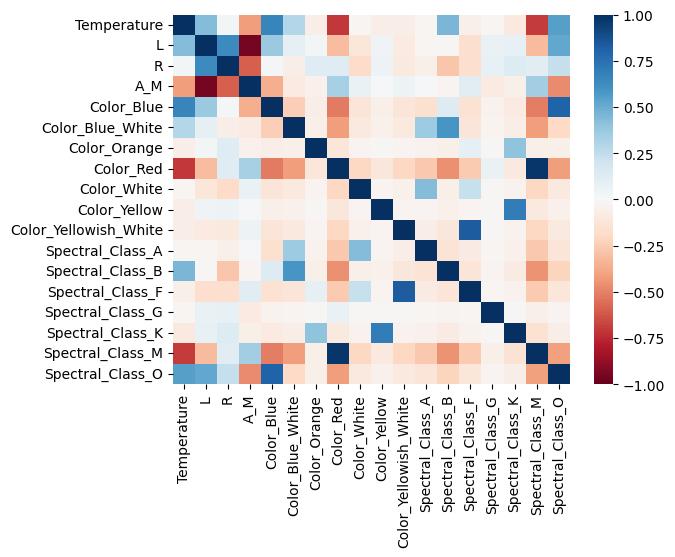
\includegraphics[width=.6\linewidth]{figures/correlation_heatmap.png}
% \end{figure}
